\documentclass[11pt,a4paper,titlepage]{article}
\usepackage[a4paper]{geometry}
\usepackage[utf8]{inputenc}
\usepackage[english]{babel}
\usepackage{lipsum}
\usepackage{eurosym}
\usepackage{rotating}

\usepackage{amsmath, amssymb, amsfonts, amsthm, mathtools}
% mathtools for: Aboxed (put box on last equation in align envirenment)
\usepackage{microtype} %improves the spacing between words and letters

\usepackage{lipsum}
\usepackage{threeparttable}
\usepackage{tabularx}
\usepackage{multirow}
\usepackage{booktabs}
\newcommand{\tabitem}{~~\llap{\textbullet}~~}
\usepackage{graphicx}
\graphicspath{ {./figures/} {./eps/}}
\usepackage{epsfig}
\usepackage{epstopdf}
\usepackage{verbatim}
\usepackage{textcomp}
\usepackage{tikz}
\usetikzlibrary{shapes,arrows}

%%%%%%%%%%%%%%%%%%%%%%%%%%%%%%%%%%%%%%%%%%%%%%%%%%
%% COLOR DEFINITIONS
%%%%%%%%%%%%%%%%%%%%%%%%%%%%%%%%%%%%%%%%%%%%%%%%%%
 % Enabling mixing colors and color's call by 'svgnames'
%%%%%%%%%%%%%%%%%%%%%%%%%%%%%%%%%%%%%%%%%%%%%%%%%%
\definecolor{MyColor1}{HTML}{CC0000} %mix personal color
\newcommand{\textb}{\color{Black} \usefont{OT1}{lmss}{m}{n}}
\newcommand{\blue}{\color{MyColor1} \usefont{OT1}{lmss}{m}{n}}
\newcommand{\blueb}{\color{MyColor1} \usefont{OT1}{lmss}{b}{n}}
\newcommand{\red}{\color{LightCoral} \usefont{OT1}{lmss}{m}{n}}
\newcommand{\green}{\color{Turquoise} \usefont{OT1}{lmss}{m}{n}}
%%%%%%%%%%%%%%%%%%%%%%%%%%%%%%%%%%%%%%%%%%%%%%%%%%


%%%%%%%%%%%%%%%%%%%%%%%%%%%%%%%%%%%%%%%%%%%%%%%%%%
%% FONTS AND COLORS
%%%%%%%%%%%%%%%%%%%%%%%%%%%%%%%%%%%%%%%%%%%%%%%%%%
%    SECTIONS
%%%%%%%%%%%%%%%%%%%%%%%%%%%%%%%%%%%%%%%%%%%%%%%%%%
\usepackage{titlesec}
\usepackage{sectsty}
%%%%%%%%%%%%%%%%%%%%%%%%
%set section/subsections HEADINGS font and color
\sectionfont{\color{MyColor1}}  % sets colour of sections
\subsectionfont{\color{MyColor1}}  % sets colour of sections

%set section enumerator to arabic number (see footnotes markings alternatives)
\renewcommand\thesection{\arabic{section}.} %define sections numbering
\renewcommand\thesubsection{\thesection\arabic{subsection}} %subsec.num.

%define new section style
\newcommand{\mysection}{
\titleformat{\section} [runin] {\usefont{OT1}{lmss}{b}{n}\color{MyColor1}}
{\thesection} {3pt} {} }

%%%%%%%%%%%%%%%%%%%%%%%%%%%%%%%%%%%%%%%%%%%%%%%%%%
%		CAPTIONS
%%%%%%%%%%%%%%%%%%%%%%%%%%%%%%%%%%%%%%%%%%%%%%%%%%
\usepackage{caption}
\usepackage{subcaption}
%%%%%%%%%%%%%%%%%%%%%%%%
\captionsetup[figure]{labelfont={color=MyColor1}}

%%%%%%%%%%%%%%%%%%%%%%%%%%%%%%%%%%%%%%%%%%%%%%%%%%
%		!!!EQUATION (ARRAY) --> USING ALIGN INSTEAD
%%%%%%%%%%%%%%%%%%%%%%%%%%%%%%%%%%%%%%%%%%%%%%%%%%
%using amsmath package to redefine eq. numeration (1.1, 1.2, ...)
%%%%%%%%%%%%%%%%%%%%%%%%
\renewcommand{\theequation}{\thesection\arabic{equation}}

%set box background to grey in align environment
\usepackage{etoolbox}% http://ctan.org/pkg/etoolbox
\makeatletter
\patchcmd{\@Aboxed}{\boxed{#1#2}}{\colorbox{black!15}{$#1#2$}}{}{}%
\patchcmd{\@boxed}{\boxed{#1#2}}{\colorbox{black!15}{$#1#2$}}{}{}%
\makeatother
%%%%%%%%%%%%%%%%%%%%%%%%%%%%%%%%%%%%%%%%%%%%%%%%%%

\newcommand{\DP}[1]{\textcolor{blue}{\textbf{(DP says: #1)}}}
\newcommand{\cri}[1]{\textcolor{green}{\textbf{(Cri says: #1)}}}

\makeatletter
\let\reftagform@=\tagform@
\def\tagform@#1{\maketag@@@{(\ignorespaces\textcolor{red}{#1}\unskip\@@italiccorr)}}
\renewcommand{\eqref}[1]{\textup{\reftagform@{\ref{#1}}}}
\makeatother
\usepackage[hidelinks]{hyperref}

%% LISTS CONFIGURATION %%
\usepackage{enumitem}
\setlist[enumerate,1]{start=0}
\renewcommand{\labelenumii}{\theenumii}
\renewcommand{\theenumii}{\theenumi.\arabic{enumii}.}

\usepackage[acronym]{glossaries}

%%%%%%%%%%%%%%%%%%%%%%%%%%%%%%%%%%%%%%%%%%%%%%%%%%
%% PREPARE TITLE
%%%%%%%%%%%%%%%%%%%%%%%%%%%%%%%%%%%%%%%%%%%%%%%%%%
\title{\blue User equipment and terminals \\
\blueb With great power comes great responsibility}
\author{Davide Peron\\ Cristina Gava}
\date{\today}
%%%%%%%%%%%%%%%%%%%%%%%%%%%%%%%%%%%%%%%%%%%%%%%%%%

\begin{document}
\maketitle

\tableofcontents
\clearpage

\section{Power Supply} \label{sec:power_supply}

\section{Power Management} \label{sec:power_management}
	\subsection{Wii U}
		The Wii U transformer has a maximum output voltage of 15V and a maximum output current of 5A, so this console consumes $15\cdot 5 = 75W$ while under full load.
		\begin{figure}[ht]
			\centering
			\begin{minipage}{0.45\textwidth}
				\centering
				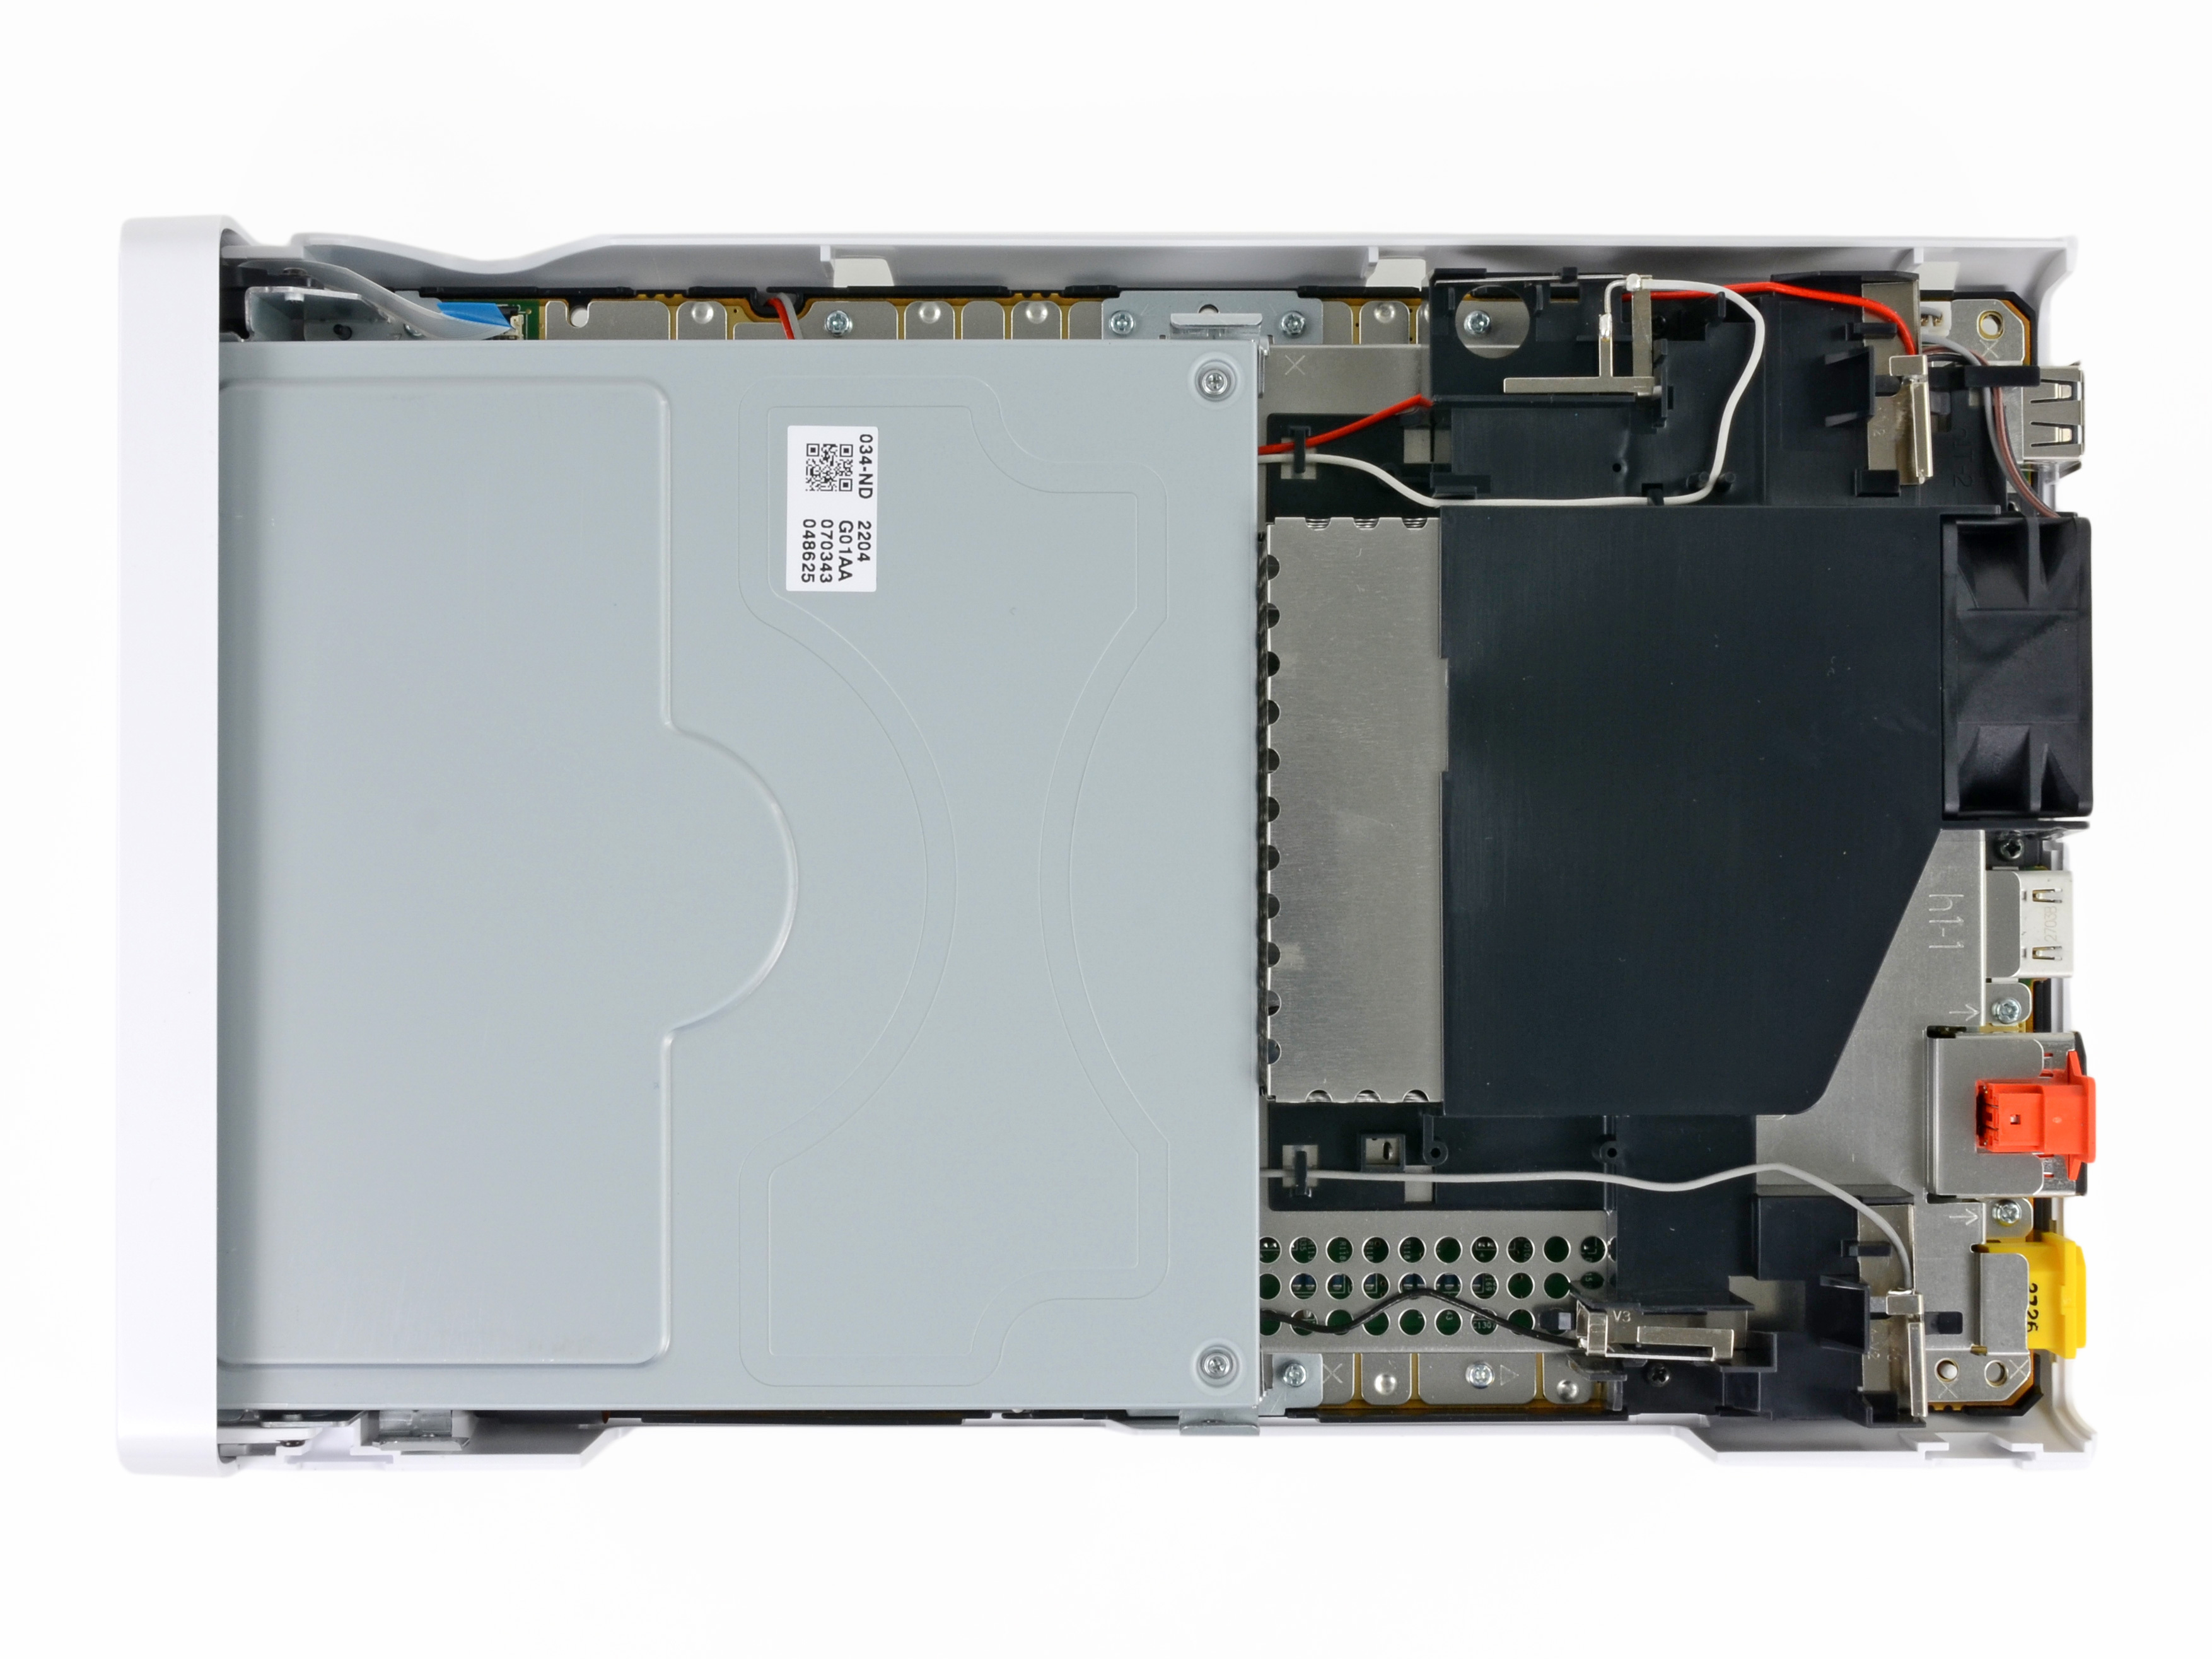
\includegraphics[width=\textwidth]{external_view.jpeg}
				\caption{Wii U without external case}
				\label{fig:external}
			\end{minipage}
			\begin{minipage}{0.45\textwidth}
				\centering
				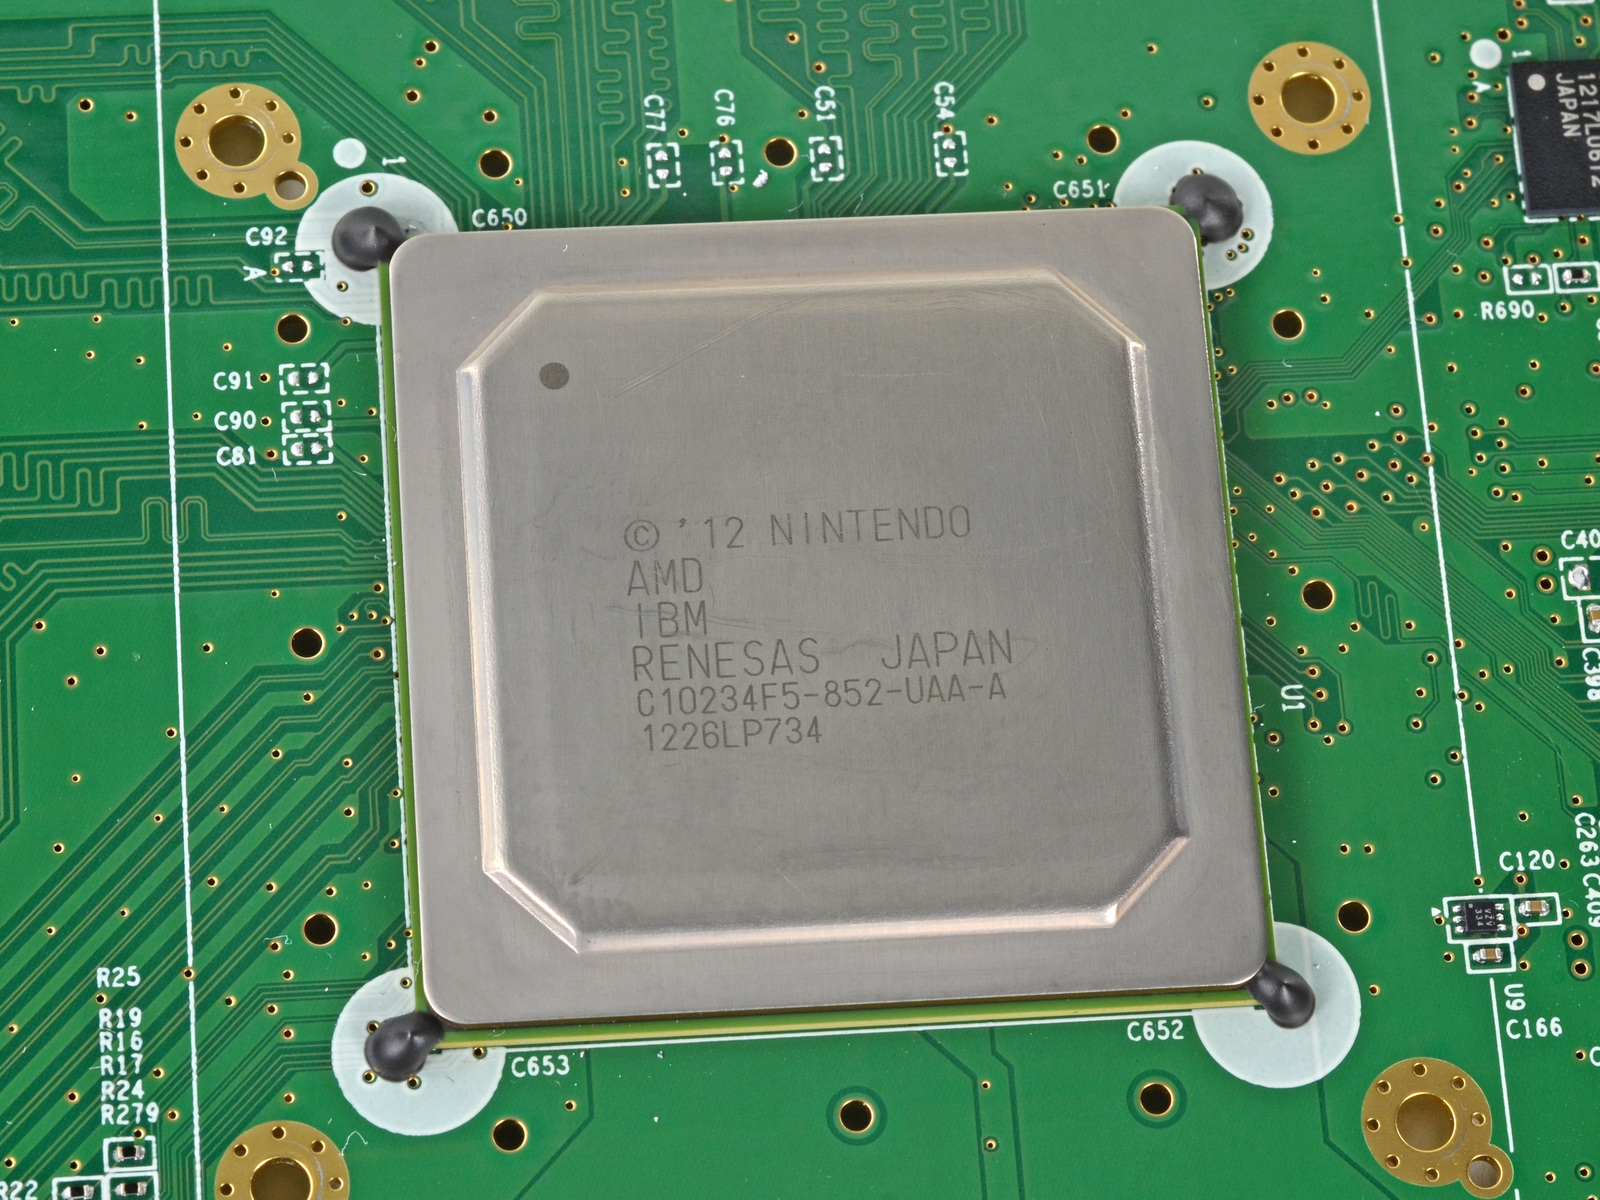
\includegraphics[width=\textwidth]{CPU_&_GPU.png}
				\caption{Wii U Multi Chip Module}
				\label{fig:mcm}
			\end{minipage}
		\end{figure}
		\begin{figure}[ht]
			\centering
			\begin{minipage}{0.45\textwidth}
				\centering
				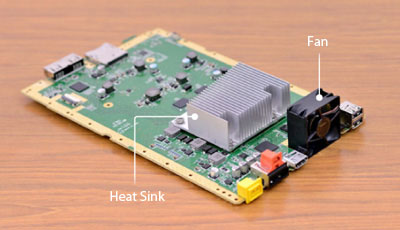
\includegraphics[width=\textwidth]{fan-heatsink.jpeg}
				\caption{Fan and heat sink position}
				\label{fig:fan-heatsink}
			\end{minipage}
			\begin{minipage}{0.45\textwidth}
				\centering
				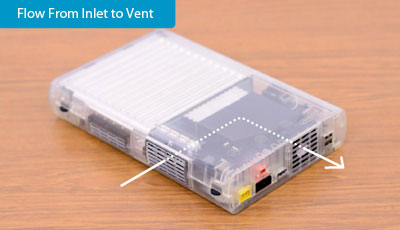
\includegraphics[width=\textwidth]{air_flow.jpeg}
				\caption{Wii U air flow demonstration}
				\label{fig:airflow}
			\end{minipage}
		\end{figure}
		In \autoref{fig:external} is shown the console without its external case.
		The first thing we note is that the bigger components inside the Wii U are the optical drive, a single heat sink used to cool down the entire console and two fans to allow the air to pass through the console.

		Analysing the position of the fan and of the heat sink, we note that the heat sink is over the main source of heat (the CPU and GPU) and it is close to the fan rotated in a way that the air can pass through it, as shown in \autoref{fig:airflow}.

		Removing the heat sink we see another thermal compound that cover both CPU and GPU. These two are put close each other maybe to reduce the latency and power consumption.

	\subsection{GamePad}
		The GamePad transformer has a maximum output voltage of 4.75V and a maximum output current of 1.6A, so this console consumes $4.75\cdot 1.6 = 7.6W$ while under full load.
\bibliographystyle{IEEEtran}
\bibliography{IEEEabrv,bibliography}

\end{document}
